%!TEX root = ../template.tex
%%%%%%%%%%%%%%%%%%%%%%%%%%%%%%%%%%%%%%%%%%%%%%%%%%%%%%%%%%%%%%%%%%%
%% chapter1.tex
%% NOVA thesis document file
%%
%% Chapter with introduction
%%%%%%%%%%%%%%%%%%%%%%%%%%%%%%%%%%%%%%%%%%%%%%%%%%%%%%%%%%%%%%%%%%%

\typeout{NT FILE chapter1.tex}%

\chapter{State of the Art}
\label{cha:state_of_the_ art}

\prependtographicspath{{Chapters/Figures/Covers/}}

% epigraph configuration
\epigraphfontsize{\small\itshape}
\setlength\epigraphwidth{12.5cm}
\setlength\epigraphrule{0pt}


\includegraphics[width=0.1\linewidth]{NOVAthesisFiles/Images/novathesis-insignia}\hfill

\includegraphics[width=0.875\linewidth]{NOVAthesisFiles/Images/novathesis-text}

\noindent This is the \gls{novathesis} \LaTeX\ template \ntindex[Template!]{Version} \novathesisversion\ from   {Template!date}\novathesisdate.

\epigraph{
  This work is licensed under the \href{https://www.latex-project.org/lppl/lppl-1-3c/}{\LaTeX\ Project Public License v1.3c}.
  To view a copy of this \ntindex[Template!]{license}, visit the \href{https://www.latex-project.org/lppl/}{LaTeX project public license}.
}


This chapter establishes the theoretical framework for the development of a distributed controller communication tool. It begins with an exploration of Petri nets, which are foundational in modeling the interactions and behavior of distributed systems. Following this, the chapter discusses GALS (Globally Asynchronous, Locally Synchronous) communication technologies, highlighting their significance in enabling efficient and reliable communication within distributed systems. The discussion then examines various communication protocols, including I2C, SPI, UART, RS-485 and FIFO with hanshake, evaluating their suitability and ensuring effective communication within the distributed IOPT controller system .Finally, the chapter introduce the IOPT-Tools environment, focusing on its role in supporting the design and development of the distributed controller communication tool.

\section{Petri Nets}
\label{sec:petri_nets}


\subsection{History}
\label{subsec:history}
The German computer scientist Carl Adam Petri formalized the concept of  Petri nets, as a formalism for modeling distributed and concurrent systems, in his 1962 PhD dissertation, \emph{Kommunikation mit Automaten}, at the Technical University of Darmstadt~\cite{adamCarlPetri}, in the following years, the theoretical foundations of Petri nets were strengthened by seminal results on decision problems such as reachability and liveness~\cite{murata}, while the annual International Conference on Applications and Theory of Petri Nets and Concurrency provided a forum to advance both theory and practice~\cite{ICPN1980}, firmly establishing Petri nets as a formal graphical language for discrete‐event and concurrent systems modeling~\cite{WikiPetriNet2025}.


In subsequent decades, the theoretical foundations of Petri nets were strengthened by seminal results on decision problems such as reachability and liveness~\cite{murata}, while the establishment of the International Conference on Applications and Theory of Petri Nets and Concurrency created an annual forum to advance both theory and practice~\cite{ICPN1980}, firmly establishing Petri nets as a formal graphical language for discrete‐event and concurrent systems modeling~\cite{WikiPetriNet2025}.

\subsection{Definition}
\label{subsec:definition}



Petri nets are a bipartite directed‐graph formalism comprising of primitive elements, \emph{places} (depicted as circles), \emph{transitions} (depicted as bars) and \emph{Arcs} (depicted as arrows), and \emph{tokens} that reside in places to represent system state (see Figure~\ref{fig:petri_diagrama}). The minimality of these primitives enables the construction of richer constructs (e.g., forks, joins) while preserving analytical tractability~\cite{50-years}. Semantically, places model local conditions or resources and transitions denote events whose firing consumes and produces tokens, thereby capturing concurrency, synchronization, conflict and choice within a unified mathematical framework~\cite{50-years}. 

Graphically, Petri nets serve as intuitive visual‐communication aids for stakeholders, such as clients, manufacturers and users, supporting model comprehension and system specification~\cite{pn-Wolfgang}.

 Mathematically, they admit formalisms like state equations and algebraic invariants for rigorous analysis; however, there is a critical tradeoff between modeling generality and analysis capability, often necessitating application‐specific restrictions or tool support for simulation and verification~\cite{murata}.


\begin{figure}[htbp]
  \centering
  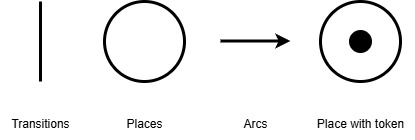
\includegraphics[width=0.6\textwidth]{Chapters/Figures/petri_image.jpg}
  \caption{Petri net elements.}
  \label{fig:petri_diagrama}
\end{figure}



The formal definition of a Petri net states that a Petri net \( PN \) is defined as the tuple (meaning they cannot be modified once created) \( PN = (P, T, F, W, M_0) \)~\cite{murata}, where:


\begin{itemize}
    \item \( P = \{ p_1, p_2, p_3, \ldots, p_m \} \) is the set of \( m \) places;
    \item \( T = \{ t_1, t_2, t_3, \ldots, t_n \} \) is the set of \( n \) transitions;
    \item \( F \subseteq (P \times T) \cup (T \times P) \) is the set of arcs representing the flow relation;
    \item \( W : F \to \{1,2,3,\ldots\} \) is the arc weight function;
    \item \( M_0 : P \to \{0,1,2,3,\ldots\} \) is the initial marking;
    \item \( P \cap T = \emptyset \) and \( P \cup T \neq \emptyset \).
\end{itemize}

A Petri net structure \( N = (P, T, F, W) \) without an initial marking is denoted by \( N \) and a Petri net with an initial marking is denoted by \( (N, M_0) \).


Figure~\ref{fig:petrinet} illustrates the interaction between two components modeled using an IOPT net. This example, taken directly from~\cite{example}, presents a Petri net incorporating a synchronous communication channel.

\begin{figure}[htbp]
  \centering
  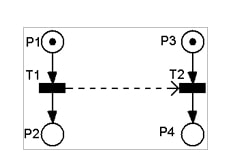
\includegraphics[width=0.6\textwidth]{Chapters/Figures/petrinet.jpg}
  \caption{Example of Petri net.}
  \label{fig:petrinet}
\end{figure}

\section{\emph{Input-Output Place-Transition} Petri Nets}
\label{sec:iopt_petri_nets}


Petri nets, over the years, have been developed and adapted to better suit different applications,  Colored Petri Nets (CPNs), Timed Petri Nets, Hierarchical Petri Nets among others were introduced to better meet these needs. The \textbf{Input-Output Place-Transition (IOPT) Petri Nets} were created to model controllers interacting with external environments through the use of input and output (I/O) interfaces\cite{iopttools}. They are considered \emph{non-autonomous}  where non-autonomous means that external signals can enable or disable transitions \cite{2015gomes}. The incorporation of inputs and output signals in Petri nets enables precise representation of the interactions between a controller and its external environment, therefore enabling its applicability in real-world environments  and making them particularly useful in automation and embedded systems\cite{iopttools}.


The IOPT framework can be defined as a tuple of input signals (IS), input events (IE), output signals (OS), and output events (OE). This design ensures the synchronization of the modeled control logic with the external environment \cite{iopttools}. The introduction of priority attributes for transitions and the inclusion of test arcs represent notable advancements over earlier versions of IOPT nets, such as those described in previous works in~\cite{barros2004} and~\cite{bg2005}. The introduction off prioritization allows for effective conflict resolution among transitions, while test arcs facilitate the implementation of fair arbitration mechanisms~\cite{conflict}.

Furthermore, the IOPT framework incorporates features such as time domains and communication channels, which support the modeling of networked controllers and globally-asynchronous locally-synchronous (GALS) systems. Its metamodel complies with the Petri Net Markup Language (PNML) and extends it with Ecore-based representations to capture I/O, timing, and communication aspects~\cite{iopttools}.




\subsection{IOPT Net Addition and Subtraction (Composition and Decomposition)}
\label{sub:net_addicion}

Net addition and net subtraction are fundamental operations in the IOPT Petri nets framework, they form the foundation for its adaptability in embedded and distributed systems.The combination and decomposition of two IOPT nets through synchronized transitions and shared places preserve the input/output (I/O) signal dependencies~\cite{add1}.

\begin{itemize}
    \item \textbf{Net Addition (Composition): }     
As the term suggests, net addition functions as a composition operator that integrates two IOPT net modules into a larger model, thereby facilitating the reuse of pre-validated components. Comparable to additive compositionality~\cite{add2}, this operation transforms submodels into coherent systems while preserving semantic consistency through synchronized transitions and shared places, which maintain the dependencies of input/output (I/O) signals~\cite{add1}.
\end{itemize}

\begin{itemize}
    \item \textbf{Net Subtraction (Decomposition): }     
Net Subtraction refers to the deliberate removal of specific subnets from a larger Petri net model without compromising the integrity of the overall system. It enables us to decompose the system into smaller, more manageable units, thereby supporting modular design approaches and  allowing for incremental development and analysis~\cite{Barrosadd}. 


In net splitting operation it is essential to identify and validate the nodes, know as the \emph{cutting set}, where the model should be broken. The validity of a cutting set is determined by adhering to the following three rules~\cite{apresentacao}:

\begin{enumerate}
    \item The cutting node is a place.
    \item The cutting node is a transition with incoming arcs exclusively from a single component.
    \item The cutting node is a transition with incoming arcs from multiple components.
\end{enumerate}

These rules ensure that the resulting submodels maintain the structural and behavioral integrity of the original system.



\begin{figure}[htbp]
  \centering
  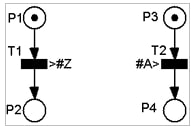
\includegraphics[width=0.6\textwidth]{Chapters/Figures/petrisplit.jpg}
  \caption{Example of Petri net after net subtraction.}
  \label{fig:petrisplit}
\end{figure}


\end{itemize}


Figure~\ref{fig:petrisplit} presents two Petri nets resulting from the decomposition of the Petri net shown in Figure~\ref{fig:petrinet}. The left-hand side have an output \( z \), while the right-hand side illustrates an input \( A \). Performing a net composition (addition) of these two subnets yields the original net represented in Figure~\ref{fig:petrinet}.


\section{GALS}
\label{sec:gals}


The increasing complexity of embedded and distributed systems necessitates modeling approaches that can effectively handle concurrency, modularity, and varying timing constraints. GALS architectures address these needs by allowing system components to operate synchronously within themselves while communicating asynchronously with other components. When integrated into the IOPT Petri net framework, GALS architectures enable a structured and scalable approach to system design and verification.

In GALS (Globally Asynchronous, Locally Synchronous) systems, each local component operates synchronously with respect to its own local clock, which governs its state evolution. However, since each component resides in a distinct clock domain, the overall system exhibits asynchronous behavior. Inter-component communication can be facilitated through asynchronous wrappers, such as those proposed in~\cite{galsborman}.


An extension of GALS systems applied to IOPT models is presented in~\cite{galsactd}, where the author introduces an attribute that specifies the Time Domain (TD) of each node within the IOPT Petri net, including both places and transitions. This attribute enables the association of each node with a specific hardware or logical component, thereby facilitating modular and time-partitioned system design.
To support communication between components operating in different time domains, the model incorporates the concept of Asynchronous Channels (ACs). An AC connects two transitions that belong to distinct time domains, for example, one acting as the master, responsible for sending events, and the other as the slave, which receives them. These events are transmitted across the AC, enabling coordinated yet asynchronous interaction between independently clocked components.


An IOPT Petri net extended with Time Domains and Asynchronous Channels can be formally defined as follows:

\begin{equation}
\text{IOPT\_GALS} = (\text{IOPT}, \text{ACs}, \text{TDs})
\end{equation}

where:
\begin{enumerate}
    \item \textbf{IOPT} denotes an IOPT Petri net, defined as in~\cite{iopttools};
    \item \textbf{ACs} is the set of asynchronous channels;
    \item \textbf{TDs} is the set of time domains.
\end{enumerate}

An IOPT net is formally defined as:
\begin{equation}
\text{IOPT} = (P, T, A, TA, M, weight_T, weight_P, priority, isg, ie, oe, osc)
\end{equation}

The following constraints further define the IOPT-GALS structure:

\begin{equation}
ACs \subseteq T \times T
\end{equation}

\begin{equation}
t_s \times t_m \subseteq ACs
\end{equation}

\begin{equation}
TDs = TDs_p \cup TDs_t \cup TDs_{ac}
\end{equation}

\noindent where \( t_m \) and \( t_s \) denote the master and slave transitions, respectively, such that:
\[
t_m \in T, \quad t_s \in T, \quad t_m \neq t_s
\]

\noindent The mapping functions are defined as:
\[
TDs_p : P \rightarrow \text{IN}, \quad TDs_t : T \rightarrow \text{IN}, \quad TDs_{ac} : ACs \rightarrow \text{IN}
\]



The integration of GALS into IOPT Petri nets involves decomposing a global system model into locally synchronous modules that communicate asynchronously. This decomposition creates TD and AC, it facilitates modular design, enabling each module to operate at its own pace without the need for global synchronization, thus improving scalability and flexibility \cite{moutinho2011petri}.




Figure~\ref{fig:petrigals} illustrates an example of a GALS system. The model depicts two distinct time domains: one on the left side (\( TD_1 \)) and another on the right side (\( TD_2 \)). Positioned between them is an asynchronous channel (AC), which facilitates communication across time domains. 

All elements on the left side operate synchronously within \( TD_1 \), while those on the right side operate synchronously within \( TD_2 \). Components sharing the same time domain communicate synchronously. However, communication between components in \( TD_1 \) and \( TD_2 \) is asynchronous and is mediated by the AC, which is associated with its own independent time domain.




\begin{figure}[htbp]
  \centering
  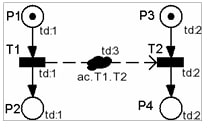
\includegraphics[width=0.6\textwidth]{Chapters/Figures/petrigals.jpg}
  \caption{Example of Petri net with GALS system.}
  \label{fig:petrigals}
\end{figure}



\section{Communication support technologies}
\label{sec:communication_support_technologies}

In this section, various communication technologies utilised within Globally Asynchronous Locally Synchronous (GALS) systems are examined. The analysis focuses on their design considerations, performance trade-offs, and integration challenges. By providing a comprehensive overview of these mechanisms, the chapter aims to equip readers with the knowledge necessary to navigate the complexities of modern integrated circuit development and to harness the benefits of GALS architectures for optimised system performance and reliability.


\subsection{I\textsuperscript{2}C}
\label{subsub:i2c}

The I\textsuperscript{2}C  (Inter-Integrated Circuit) protocol is described as a multi-master, serial and single-ended bus that requires only two lines for communication: the clock line (SCL) for synchronization and the data line (SDA) for transmitting information. This simplicity is underscored by the minimal hardware requirements, just three connections (SCL, SDA, and GND), making it an ideal choice for connecting the central controller (master) with multiple local controllers (slaves) \cite{i2c}.

Despite its advantages, the I\textsuperscript{2}C  protocol presents certain limitations that may hinder its suitability for high-performance or large-scale applications. The standard I\textsuperscript{2}C bus supports data rates of up to 3.4 Mbps in high-speed mode, which may prove inadequate for systems that demand greater throughput. Moreover, the inherent bus capacitance imposes constraints on the number of connected devices, the permissible bus length and may have problems with bus contention, thereby limiting the scalability of the system ~\cite{I2Cv2}.

I\textsuperscript{2}C is a synchronous communication protocol that requires a shared clock signal between the master and slave devices. Since I\textsuperscript{2}C assumes that both devices operate within the same clock domain, it is not suitable for the asynchronous components of GALS (Globally Asynchronous, Locally Synchronous) systems. However, it can be considered for use within the locally synchronous parts of such systems.

\subsection{SPI}
\label{subsub:spi}

The Serial Peripheral Interface (SPI) protocol operates in Full-Duplex mode, allowing simultaneous data transmission and reception this aligns well with the requirements of GALS architectures~\cite{spisite}. Same as other serial protocols it has a master-slave configuration with a central module (master) to coordinate communication, ensuring data integrity across asynchronous boundaries. It uses four primary lines for communication. These signals include SCK (Serial Clock), MOSI (Master Output Slave Input), MISO (Master Input Slave Output), and SS (Slave Select). The protocol's simplicity and high-speed data transfer rates, often ranging from 10 Mbps to several tens of Mbps, make it suitable for applications demanding rapid and reliable data exchange adding ~\cite{spisite}.

The protocol’s inherent simplicity, flexibility, and capacity for high-speed data transfer, often ranging from 10 Mbps to several tens of Mbps, render it well-suited for applications requiring rapid and reliable data exchange. Additionally, its ability to simultaneously transmit and receive data, coupled with support for multiple slave devices through individual Slave Select (SS) lines, facilitates scalable system designs.

While the Serial Peripheral Interface (SPI) protocol offers several advantages, it also presents notable limitations. Each additional slave device requires a dedicated Slave Select (SS) line, which can increase the pin count on the master device and complicate hardware design, particularly in systems with numerous peripherals. Moreover, unlike protocols such as  I\textsuperscript{2}C, SPI does not include inherent error-checking mechanisms, necessitating the implementation of additional measures to ensure data integrity. Furthermore, SPI is typically optimized for short-distance communication within a single printed circuit board (PCB), as signal degradation and timing issues may arise over extended distances. These factors can limit the scalability and robustness of SPI in more complex or distributed system architectures~\cite{spisite2}.


SPI, like I\textsuperscript{2}C, is a synchronous communication protocol, meaning that data transmission is synchronized by a clock signal generated by the master device. Although this ensures reliable data transfer, SPI is only suitable for the synchronous parts within a GALS (Globally Asynchronous, Locally Synchronous) subsystem and is not appropriate for communication between asynchronous GALS domains.

\subsection{UART}
\label{sub:uart}

The Universal Asynchronous Receiver-Transmitter, UART, is a fundamental component in serial communication systems, particularly in embedded and microcontroller-based applications ~\cite{UARTwiki}. It is a hardware asynchronous communication with full-duplex data exchange using two or four signal lines. In its two-signal configuration, communication is carried out via the transmit (TX) and receive (RX) lines. In the four-signal variant, additional control signals, ready-to-send (RTS) and clear-to-send (CTS), are included to enable hardware-based handshaking for improved flow control~\cite{Rao2021}.

UART operates by converting parallel data into serial form for transmission, and performing the reverse operation during reception. The data frame typically includes a start bit (logical low), a defined number of data bits, an optional parity bit for error detection, and one or more stop bits. While UART handles data framing and signal generation, it does not define a standardized signaling protocol between devices, requiring both ends to be properly configured. UART signals are output at the operating voltage of the device, making them suitable for short-range communication between components operating at identical voltage levels. However, in many practical applications, this condition is not met, for this reason  UART signals are often routed through line drivers to convert them into standard electrical signaling formats, such as RS-485, to support longer distances and improve noise immunity~\cite{Rao2021}.

UART communication does not rely on a shared clock signal, instead communicating devices uses predefined baud rates to determine the timing of data bits to ensure synchronization ~\cite{UARTard}.  The integration of UART modules within IOPT Petri net models is crucial for the accurate representation and verification of asynchronous communication in GALS systems. 




\subsection{FIFO + Handshake}
\label{sub:fifo+handshake}

A small asynchronous FIFO buffer holds data between the sensor and robotic arm controller.

Handshake signals (valid / ready or req / ack) control safe data transfer.

This ensures:

No data is lost or overwritten.

Timing mismatch between the two systems is tolerated.

Very efficient
 Fully decouples sender and receiver
Ideal for FPGA or hardware-in-the-loop systems

\section{IOPT tools}
\label{sec:iopt_tools}



The theoretical constructs of IOPT Petri nets (Section~\ref{sec:iopt_petri_nets}) and the principles of GALS architectures (Section~\ref{sec:gals}) find practical application in controller design through specialized software environments. One such comprehensive platform is IOPT-Tools, an integrated, web-based development environment tailored for the design, verification, and implementation of embedded system controllers, particularly for industrial automation and digital systems~\cite{iopttools}. As previously mentioned~\cite{iopttools}, IOPT-Tools supports a model-driven development workflow, starting from graphical Petri net model creation to verification and, crucially for this work, automatic code generation in C or VHDL.

The environment's capacity to handle complex systems is partly due to its support for IOPT Petri net characteristics, including the input and output mechanisms essential for controller interaction and features facilitating model modularity, such as the net decomposition operations discussed in Section~\ref{sub:net_addicion}. These operations allow a complex controller model to be broken down into several distinct sub-models, which can then be targeted for execution on separate computational nodes, aligning with the distributed control paradigm.


In addition to design and verification, IOPT-Tools includes automatic code generation capabilities, enabling the creation of software in C or hardware descriptions in VHDL~\cite{vhld}. This feature streamlines the transition from design to deployment, allowing for efficient and error-free implementation of the controller in either software or hardware~\cite{manual}.

IOPT-Tools delivers a complete, start-to-finish solution for creating controllers for embedded systems. The integration of graphical design, formal verification, and automatic code generation within a single, web-based platform significantly increases efficiency, reliability, and speed of controller development for both industrial and digital applications.


\subsection{Highlighting the Communication Gap}
\label{subsec:communication_gap}

While IOPT-Tools provides this extensive support for developing and generating code for individual controller logic, and facilitates the decomposition of models for distributed architectures, a significant challenge remains in automatically establishing and managing the communication between these distributed sub-models. The current automatic code generation primarily focuses on the internal logic of each individual sub-model. Crucially, it does not extend to automatically generating the necessary communication infrastructure required for these distinct sub-models to interact efficiently and reliably when deployed across different computational nodes.

This lack of automated support for diferent sub models, or petri nets, communication means that engineers must currently undertake the complex and error-prone task of manually implementing these communication links. This manual process involves selecting appropriate communication technologies (such as those reviewed in Section~\ref{sec:communication_support_technologies}), writing and integrating low-level driver code, and ensuring data consistency. This not only diminishes the benefits of automated generation for the core logic but also increases development time, hinders system optimization, and introduces potential for integration issues.

Addressing this specific gap,by designing and implementing a tool that automates the generation of code for efficient and reliable communication channels between distributed IOPT sub-models, is the central objective of this dissertation. This will further enhance IOPT-Tools' capabilities for developing truly distributed control systems.


\subsection{Overview of Key Components in IOPT-Tools}
\label{sub:iopt_tools_components}

talk about graphical editor, verification engine, existing code generator (and its limitations)






